
\documentclass{abgabe}

\begin{document}
\begin{questions}
    \qformat{\thequestion. \textbf{\thequestiontitle} \hfill}
    \titledquestion{Sequenzdiagramm: Wetterstation}

    In der Vorlesung haben Sie das Observer Pattern (zu deutsch Beobachter Entwurfsmuster) am Beispiel einer Wetterstation kennengelernt.
    Als Beispiel für konkrete Implementierungen der Interfaces Subject und Observer werden die Klassen \texttt{WeatherData} bzw. \texttt{CurrentConditionsDisplay} aus dem Foliensatz verwendet.

    Modellieren Sie in Visual Paradigm ein Sequenzdiagramm, das diesen Sachverhalt darstellt.
    Das Diagramm soll die Interaktion der Klassen für den folgenden Programmablauf modellieren:

    \begin{enumerate}
        \item Eine Wetterstation startet und erstellt jeweils eine neue Instanz der Klassen \texttt{WeatherData} und \texttt{CurrentConditionsDisplay}. (Das Display bekommt die Wetterdaten im Konstruktor übergeben und registriert sich anschließend als Observer, siehe Folien)
        \item Es treten zwei Veränderungen des Wetters auf. Modellieren Sie einen Pull oder einen Push-Observer (Orientieren Sie sich an den Folien für einen Push-Observer)
        \item Der Observer wird vom Subject entfernt.
        \item Die Wetterstation wird abgeschaltet und der Speicher wird freigegeben.
    \end{enumerate}

    \textbf{Hinweise:}

    \begin{itemize}
        \item Achten Sie zudem darauf, dass Methodenaufrufe innerhalb der selben Klasse richtig dargestellt werden.
        \item Benutzen Sie explizite Namen mit Typ für die Benennung der Teilnehmer.
        \item Benutzen Sie für Nachrichten die Form \\ \texttt{<Nachrichtenname> (<Parametername>=<Argumentwert>,...)}
    \end{itemize}

    \begin{solution}
        \begin{center}
            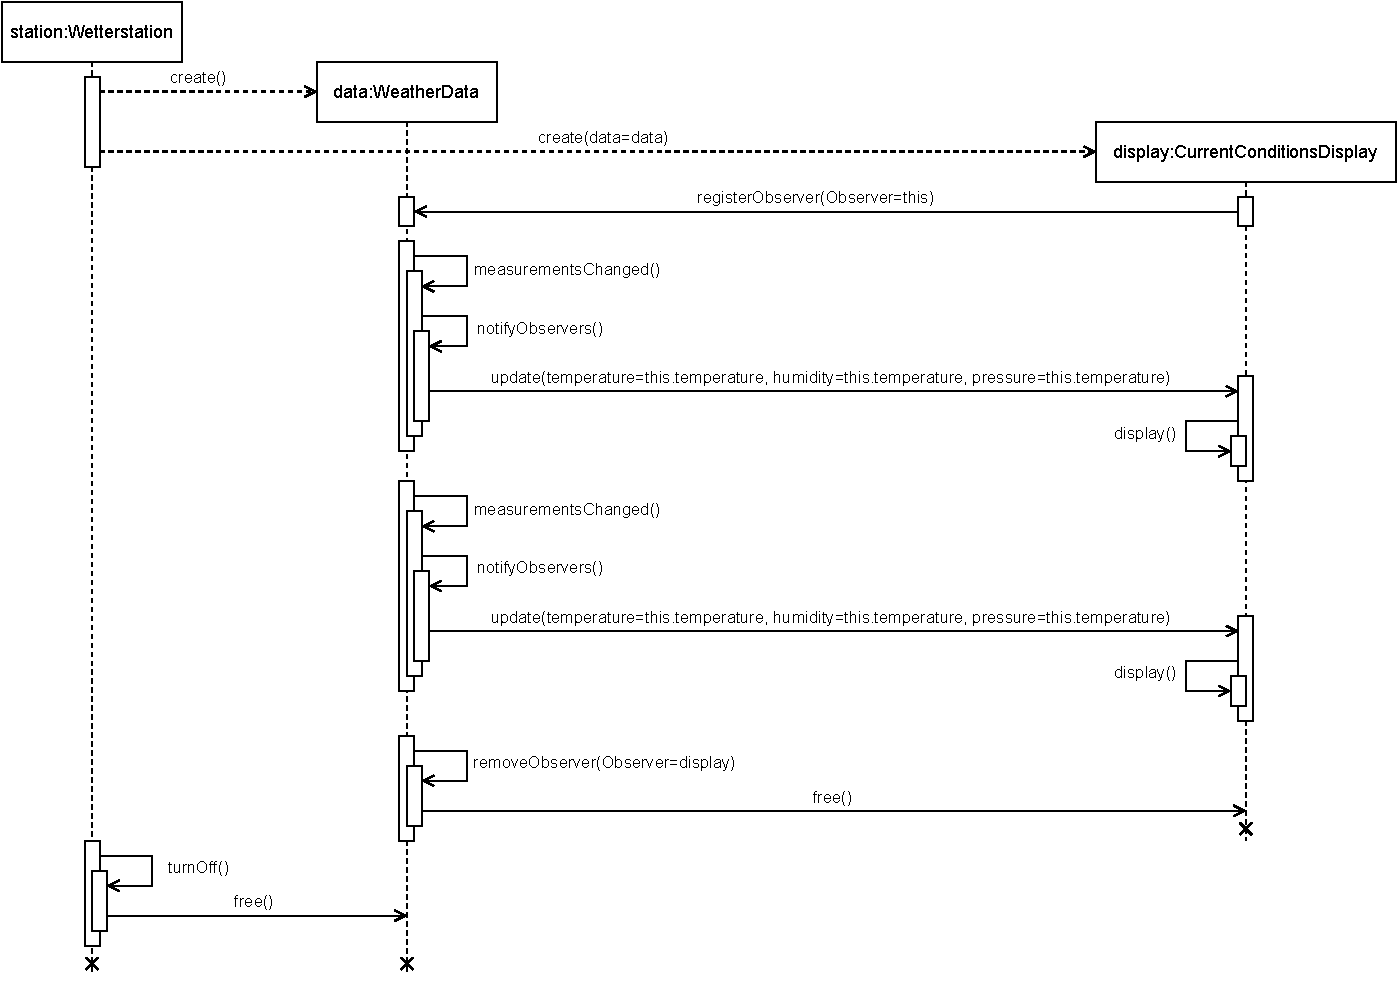
\includegraphics[width=\textwidth]{swt_h09_weather.pdf}
        \end{center}
    \end{solution}

\end{questions}

\end{document}